\documentclass[10pt,a4paper]{article}
\usepackage[utf8]{inputenc}
\usepackage[english]{babel}
\usepackage{amsmath}
\usepackage{amsfonts}
\usepackage{amssymb}
\usepackage{graphicx}
\usepackage{grffile}
\usepackage{float}
\usepackage{hyperref}
\usepackage[left=2cm,right=2cm,top=2cm,bottom=2cm]{geometry}
\usepackage{listings}
\usepackage{verbatim}
\lstset{basicstyle=\ttfamily,
  showstringspaces=false,
  commentstyle=\color{red},
  keywordstyle=\color{blue}
}
\author{Julia Desmazes}
\title{Lab1 Rasbian RT}
\begin{document}
\maketitle

\section{Latency test}
\subsection{Supported schedualing policies}
\subsection{Cyclictest}
%). The measuring threads are woken up periodically with a defined interval by an expiring timer (cyclic alarm). Subsequently, the difference between the programmed and the effective wake-up time is calculated and handed over to the master thread via shared memory. The master thread tracks the latency values and prints the minimum, maximum and average for the latency once the number of iterations specified is completed. 
Cyclictest is a programme included in the rt\_test suite to measure the latency of an particular environement. It creats a defined number of threads that it wakes up at set intervals and then measures the latency between the moment the thread was expected to wake-up and the actual time the action took place.\\
Reading the \emph{-h} guide we can learn that \emph{-t} allows us to set the number of threads we wish to create and \emph{-p} sets the priority. 
\paragraph{threads \emph{-t}}
More precisly if no parameter is give the number of threads will be equal to the number of cpus and the execution of thows threads will be ballanced equlay\footnote{under the best possible conditions} between they s different cpu's. As we are currently on a 4 cpu system if we wish to create 4 threads leaving it to the default option would be correct. But if we didn't specify the \emph{-t} option then only 1 thread would have been created.
\begin{lstlisting}[language=bash,caption={cyclictest -h}]
-t       --threads         one thread per available processor
-t [NUM] --threads=NUM     number of threads:
without NUM, threads = max_cpus
without -t default = 1
\end{lstlisting}
\paragraph{priorities \emph{-p}}
%By default threads are squeduqled with SCHED_FIFO under cyclictest
In linux priority ranges are fixed by the schedualing algorythme used. by default cyclictest runs SCHED\_FIFO\footnote{See patch for fix \url{https://www.spinics.net/lists/linux-rt-users/msg05449.html}} and it's priorities will range from 0 to 99. Here priorities are reversed with 99 beeing the highest priority and 0 the lowest.
\begin{lstlisting}[language=bash,caption={cyclictest -h}]
-p PRIO  --prio=PRIO       priority of highest prio thread
\end{lstlisting}
\subsection{Test}
\subsubsection{SHED\_OTHER}

\begin{lstlisting}[language=bash,caption={preempt-rt kernel}]
^Cpi@raspberrypi:~/rt-tests$ sudo ./cyclictest --policy=other -t -n
policy: other/other: loadavg: 0.01 0.03 0.03 1/150 1324          

T: 0 ( 1229) P: 0 I:1000 C:1242270 Min:     21 Act:   71 Avg:   69 Max:    2541
T: 1 ( 1230) P: 0 I:1500 C: 828181 Min:     21 Act:   67 Avg:   67 Max:    1991
T: 2 ( 1231) P: 0 I:2000 C: 621135 Min:     21 Act:   68 Avg:   68 Max:    4476
T: 3 ( 1232) P: 0 I:2500 C: 496909 Min:     21 Act:   67 Avg:   69 Max:    3180
\end{lstlisting}
\begin{lstlisting}[language=bash,caption={volontary kernel}]
sudo ./cyclictest -t -n

policy: other/other: loadavg: 0.31 0.09 0.02 1/116 702          

T: 0 (  695) P: 0 I:1000 C:1220752 Min:     15 Act:   66 Avg:   66 Max:     528
T: 1 (  696) P: 0 I:1500 C: 813835 Min:     15 Act:   65 Avg:   64 Max:     490
T: 2 (  697) P: 0 I:2000 C: 610376 Min:     16 Act:   66 Avg:   67 Max:    1354
T: 3 (  698) P: 0 I:2500 C: 488301 Min:     15 Act:   64 Avg:   65 Max:     545

\end{lstlisting}

\subsubsection{SHED\_FIFO}
\begin{figure}[H]
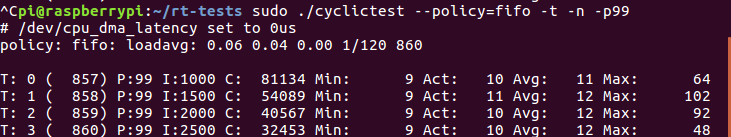
\includegraphics[width=16cm]{Voluntary-Fifo-WithoutHackbench.png}
\caption{SHED\_FIFO volontary}
\end{figure}
\begin{figure}[H]
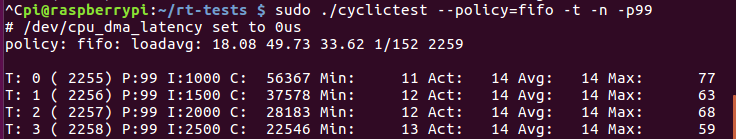
\includegraphics[width=16cm]{Preempt-Fifo-WithoutHackbench.png}
\caption{SHED\_FIFO preempt-rl}
\end{figure}
\subsubsection{SHED\_RR}
\begin{figure}[h]
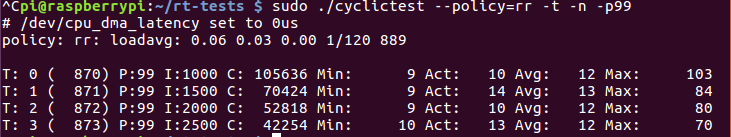
\includegraphics[width=16cm]{Voluntary-RR-WithoutHackbench.png}
\caption{SHED\_RR volontary}
\end{figure}
\begin{figure}[H]
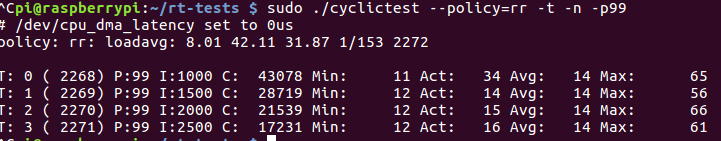
\includegraphics[width=16cm]{Preempt-RR-WithoutHackbench.png}
\caption{SHED\_RR preempt-rl}
\end{figure}
\subsubsection{Conclusion}
We observe that throughout all the diffrent scheduals have about similar avredge execution times with a slight advantage for the volontary kernel. But, we there is a muth higher maximum times for the volontary kernel than the preemptive kernel, this is because the preemptive kernel was designed to give a best worst time performance.
%Todo need shed other to conclude
\subsection{Cyclictest + Hackbench}
\subsubsection{Hackbench under SHED\_OTHER and priority 20}
\begin{figure}[H]
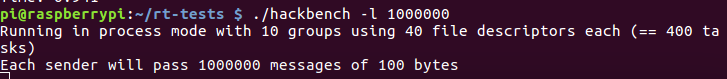
\includegraphics[width=16cm]{Volontary-other-Hackbench-p20.png}
\caption{Hackbench under SHED\_OTHER and priority 20}
\end{figure}
\subsubsection{Volontary}
\begin{figure}[H]
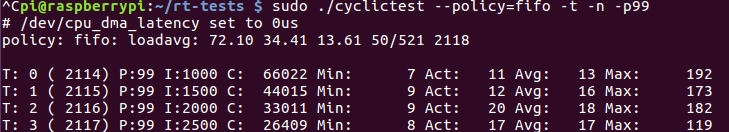
\includegraphics[width=16cm]{Volontary-Fifo-WithHackbench1.png}
\caption{Volontary fifo with hackbench}
\end{figure}
\begin{figure}[H]
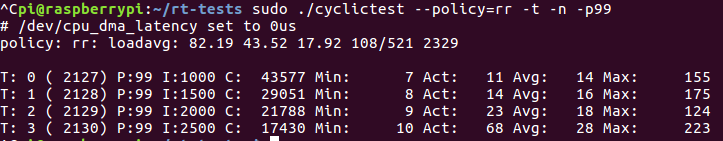
\includegraphics[width=16cm]{Volontary-Rr-WithHackbench1.png}
\caption{Volontary rr with hackbench}
\end{figure}
\subsubsection{Preempt-rt}
\begin{lstlisting}[language=bash,caption={Preempt fifo with hackbench}]
pi@raspberrypi:~/rt-tests$ sudo ./cyclictest --policy=fifo -t -n -p99
policy: fifo: loadavg: 130.65 51.20 18.86 85/551 1404           

T: 0 ( 1396) P:99 I:1000 C: 106248 Min:      7 Act:   26 Avg:   20 Max:      78
T: 1 ( 1397) P:99 I:1500 C:  70832 Min:      7 Act:   18 Avg:   20 Max:      73
T: 2 ( 1398) P:99 I:2000 C:  53124 Min:      7 Act:   24 Avg:   20 Max:      73
T: 3 ( 1399) P:99 I:2500 C:  42499 Min:      9 Act:   22 Avg:   21 Max:      74
\end{lstlisting}
\begin{lstlisting}[language=bash,caption={Preempt rr with hackbench}]
pi@raspberrypi:~/rt-tests$ sudo ./cyclictest --policy=rr -t -n -p99 
policy: rr: loadavg: 133.77 95.30 43.45 100/551 1454          

T: 0 ( 1450) P:99 I:1000 C:  70877 Min:      8 Act:   20 Avg:   20 Max:      91
T: 1 ( 1451) P:99 I:1500 C:  47251 Min:      8 Act:   20 Avg:   21 Max:      83
T: 2 ( 1452) P:99 I:2000 C:  35438 Min:      9 Act:   23 Avg:   21 Max:      69
T: 3 ( 1453) P:99 I:2500 C:  28350 Min:      9 Act:   21 Avg:   21 Max:      92
\end{lstlisting}
\subsubsection{Hackbench under RT scheduling policies and priority 49}
\paragraph{SHED\_FIFO}
\begin{figure}[H]
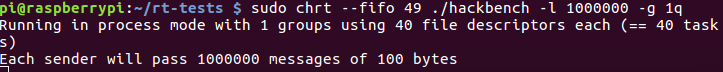
\includegraphics[width=16cm]{Hackbench2.png}
\caption{Hackbench with shed\_fifo and priority 49}
\end{figure}
\begin{figure}[H]
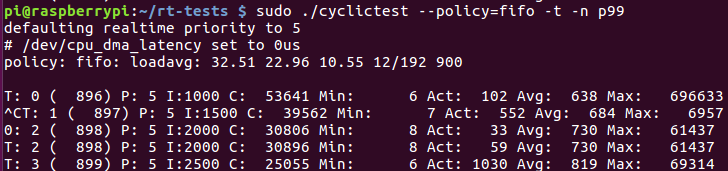
\includegraphics[width=16cm]{Preempt-Fifo-WithHackbench2.png}
\caption{Preempt-rt with fifo}
\end{figure}
\begin{figure}[H]
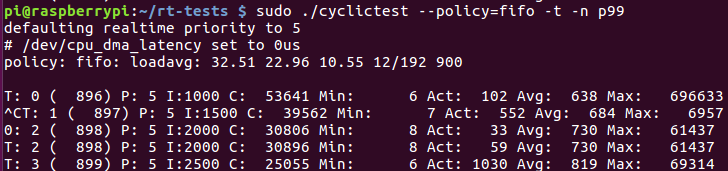
\includegraphics[width=16cm]{Preempt-Fifo-WithHackbench2.png}
\caption{Preempt-rt with fifo}
\end{figure}
\paragraph{SHED\_RR}
\begin{lstlisting}[language=bash,caption={Hackbench with shed\_rr and priority 49}]
pi@raspberrypi:~/rt-tests$ sudo chrt --rr 49 ./hackbench -l 1000000 -g 1q                     
Each sender will pass 1000000 messages of 100 bytes
\end{lstlisting}
\begin{figure}[H]
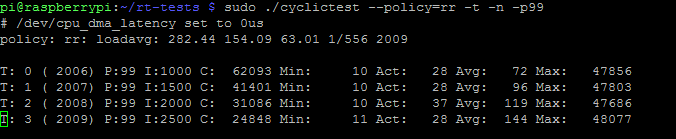
\includegraphics[width=16cm]{Preempt-RR-WithHackbench.png}
\caption{Preempt-rt with fifo}
\end{figure}
\begin{lstlisting}[language=bash,caption={Volontary kernel}]
sudo ./cyclictest --policy=rr -t -n -p99
policy: rr: loadavg: 29.39 27.96 14.37 32/161 848          

T: 0 (  832) P:99 I:1000 C: 338191 Min:      8 Act:   18 Avg:   67 Max:   49660
T: 1 (  833) P:99 I:1500 C: 225480 Min:      8 Act:   54 Avg:   96 Max:   49563
T: 2 (  834) P:99 I:2000 C: 169312 Min:      8 Act:   18 Avg:  118 Max:   49511
T: 3 (  835) P:99 I:2500 C: 135316 Min:      9 Act:   19 Avg:  144 Max:   47964
\end{lstlisting}
\section{ADA concurrent programs}
\subsection{Program 1}
\paragraph{code}
\begin{figure}[H]
\begin{center}
\verbatiminput{main.adb}
\caption{Program 1}
\end{center}

\end{figure}

\paragraph{Observations}
The A,B,C,D are printed in order throwout the execution with there not beeing any apparent modification of that ordered sequence.
\subsection{Program 2}
\paragraph{code}
\begin{figure}[H]
\begin{center}
\verbatiminput{main2.adb}
\caption{Program 2}
\end{center}
\end{figure}

\paragraph{Observations}
%Todo recall the main diffrences between the two packages and constructs
In this test we can observe that even thow both treads are confirured to sleep for the same 100ms time interval they eventually end up off sync. We can attribute this to the diffrence between the way time is treated in the \emph{delay} and \emph{delay until}.
\\
%diffrence
\subparagraph{delay}
This main diffrence is that \emph{delay} uses an \textit{approximate relative time delay}. It measured the time from a specific refrence point . If this refrence point si deisplaced in time by the process beeing preempted for example this  introduces a delay of \emph{at least} the amount of time specified,not the exact specified task. This introdoced local drift (delay) can be cumulated resulting in this unsynchronisation.
If we wanted delay to wait for an absolute time then the task would have to run uninterrupted by any other task whitch is not the case here.
\subparagraph{delay until}
This statement sheduales for an absolute wake-up task, this works by making the task not schedualable until the interval time has elapsed. Her again there is no guaranty on the actual time the task will be executed if for example the ressource required to handle that task is not available ( used by a higher priority task , ect ... ) the task will still eventually stall. 
%todo finish later 
\end{document}